This document contains the whole API specification for the BNG Bootloader project, as generated by the Doxygen documentation generator tool.

The document is built from the C sources into different formats, it's made available in HTML and PDF formats. Please refer to the project's documentation for the exact location of these documents.

The complete project (prosa) documentation is built from ReST sources using Sphinx and can be found in HTML format at the address: {\tt http://garetjax.github.com/Bootloader/}\section{Overview}\label{main_Overview}
\begin{Desc}
\item[{\bf Todo}]Move this documentation to another file or to the Sphinx documentation.\end{Desc}
Before presenting the in-\/depth API documentation, the UML diagram in Fig. 1.1 was created to present an higher-\/level overview of the API.

The {\ttfamily Controller} \char`\"{}class\char`\"{} representes our {\ttfamily main} function, and is responsible for the initialization of the various parts of the system, their respective interconnection (serial interface initialization, command registration,...) and the routing of every received command to the command dispatcher, which will in turn call the right command passing the parsed tokens as arguments.

Each command will then execute its task interacting with either the application manager or the configuration registry.

\begin{DoxyNote}{Note}

\begin{DoxyItemize}
\item Different realation graphs are automatically generated by Doxygen during the build phase, please refer to them for an in-\/dept view.
\item In the diagram below, each package representes a component, a class a C source file and the methods, the different functions contained in the file (the only exception is the {\ttfamily Command} interface, which representes the type of a command like function).
\item The details about the function prototypes where omitted for the sake of clarity.
\end{DoxyItemize}
\end{DoxyNote}
 
\begin{DoxyImage}
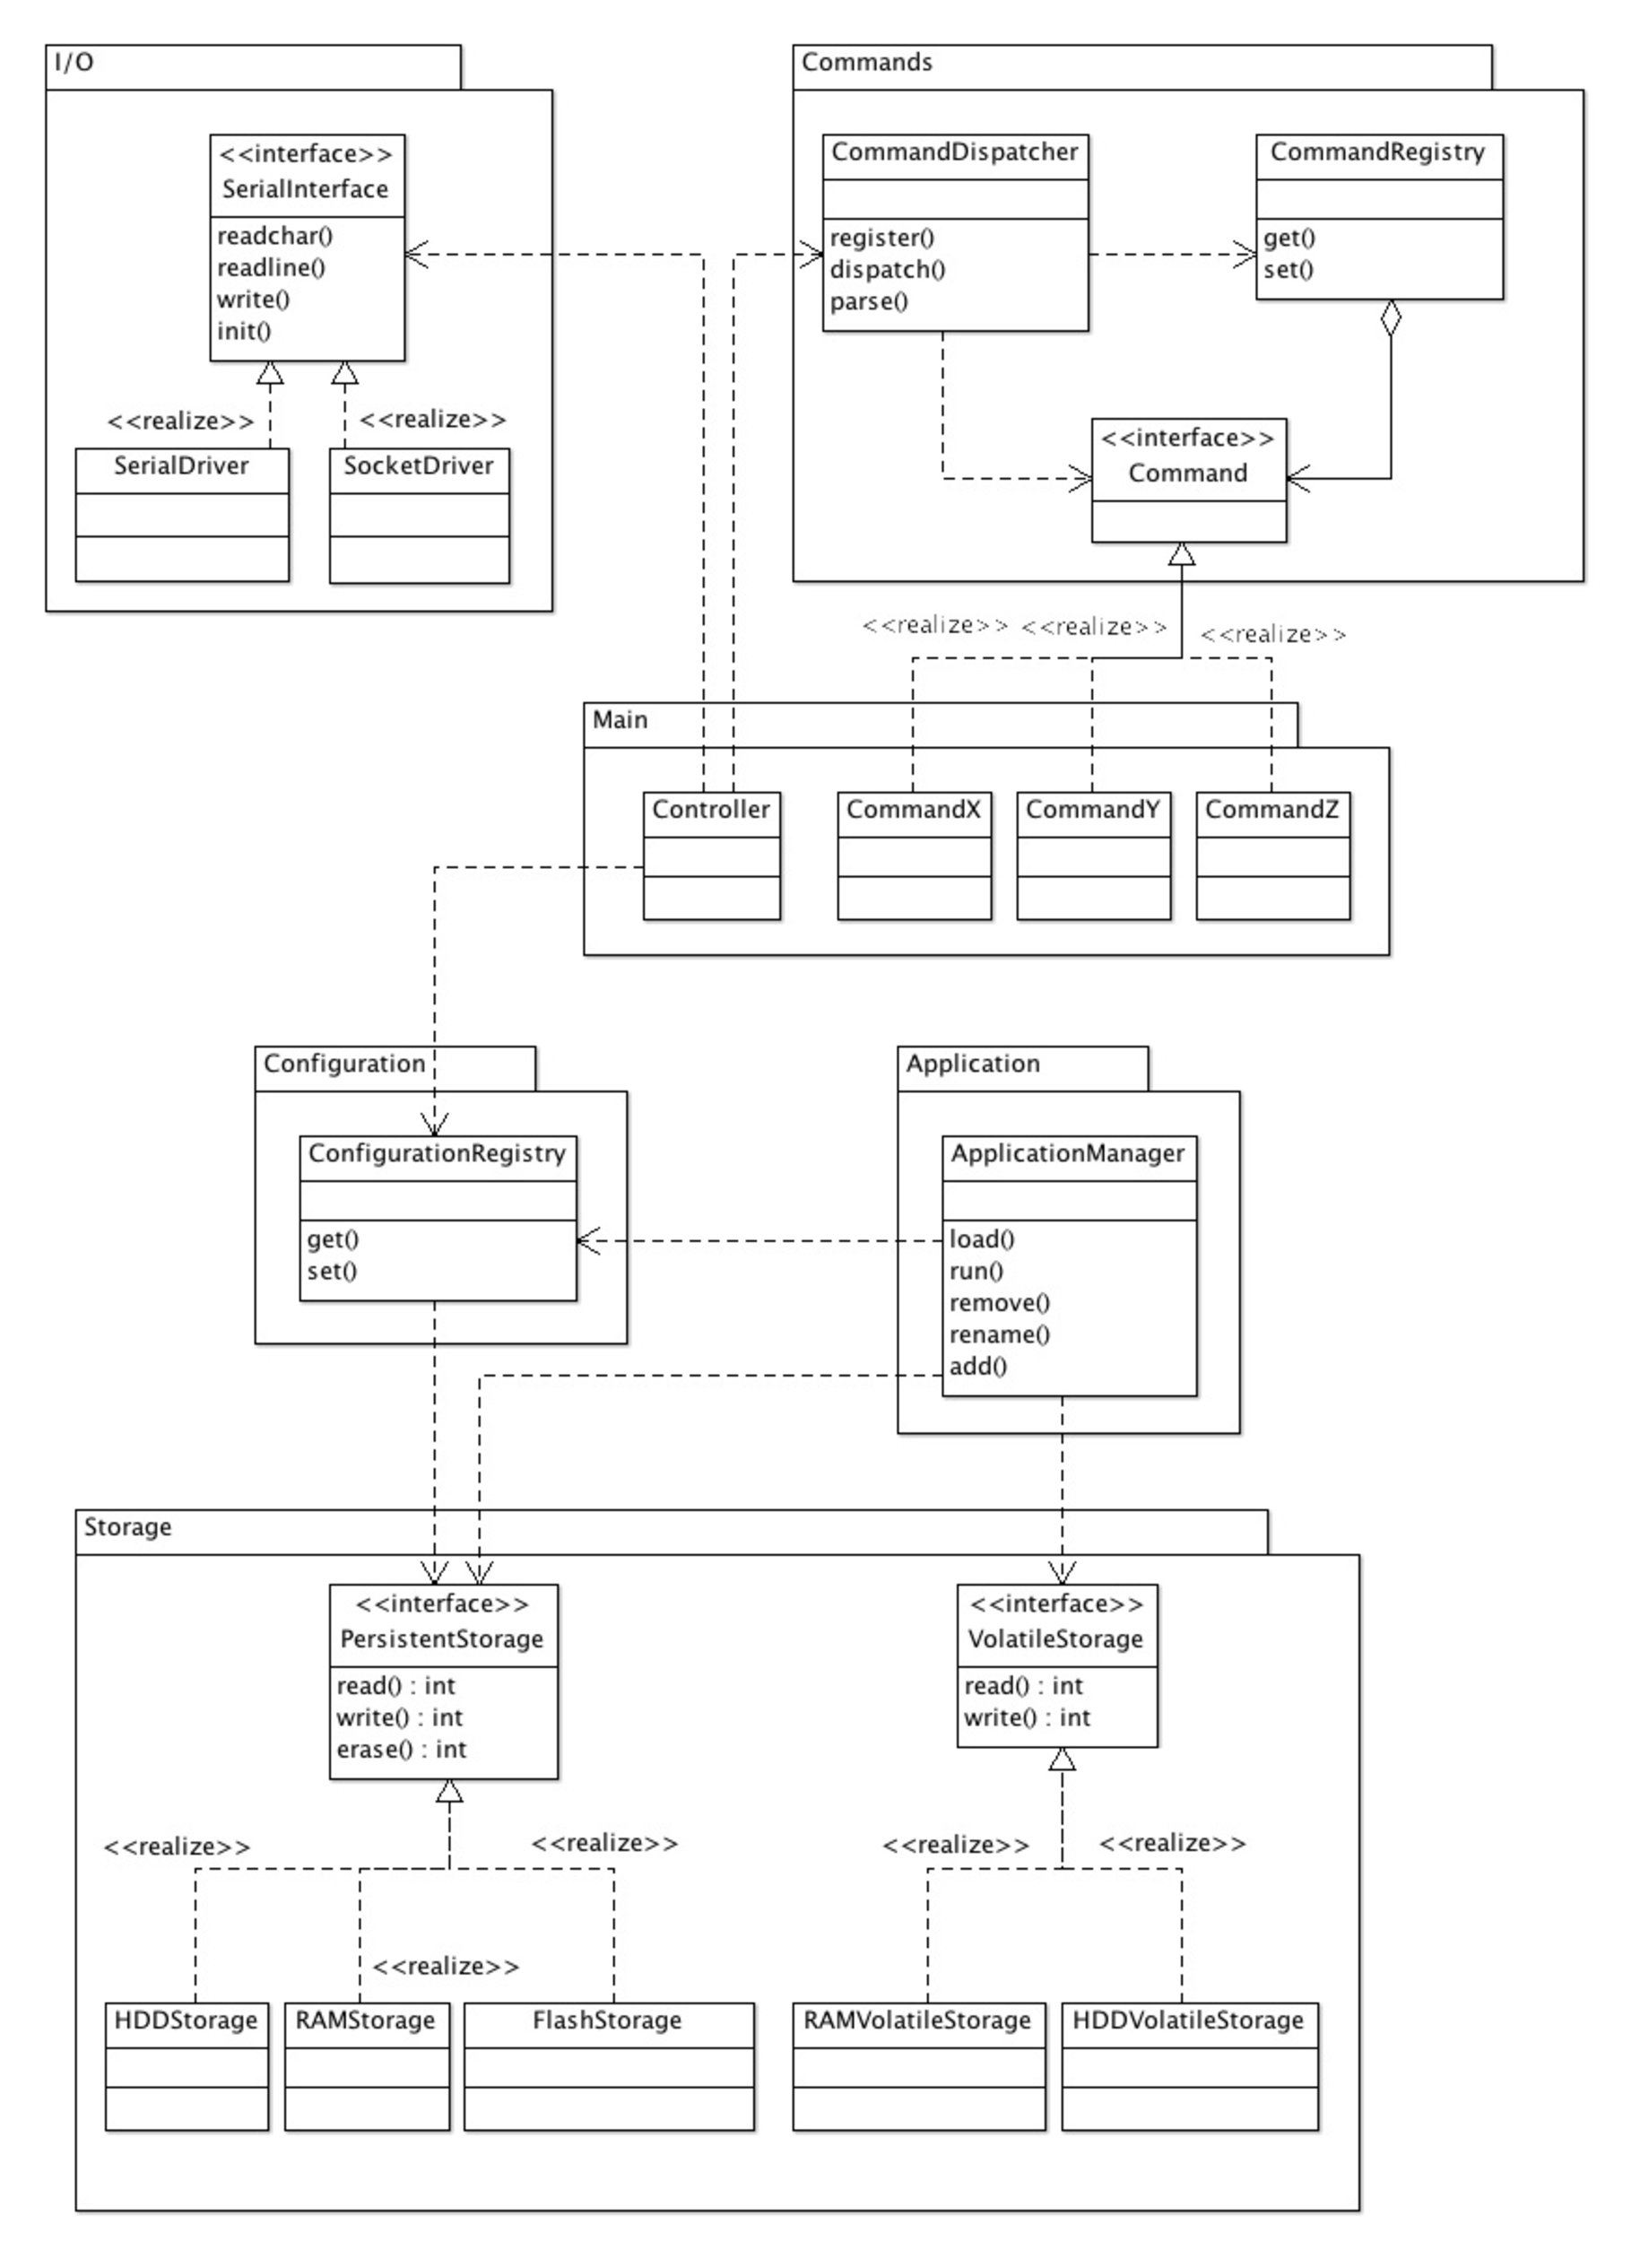
\includegraphics[width=\textwidth]{APIOverview}
\caption{API Overview}
\end{DoxyImage}
 